\documentclass[12pt]{article}

\usepackage{fullpage}
\usepackage{multicol,multirow}
\usepackage{tabularx}
\usepackage{ulem}
\usepackage[utf8]{inputenc}
\usepackage[russian]{babel}
\usepackage{graphicx}
\usepackage{indentfirst}


\begin{document}

\section*{Лабораторная работа №\,3 по курсу дискрeтного анализа: сортировка за линейное время}

Выполнил студент группы М08-207Б МАИ \textit{Цапков Александр}.

\subsection*{Условие}

\begin{enumerate}
\item Требуется разработать программу, осуществляющую ввод пар «ключ-значение»,
 их упорядочивание по возрастанию ключа указанным алгоритмом сортировки за линейное
 время и вывод отсортированной последовательности.
\item Поразрядная сортировка.

Тип ключа: MD5-суммы (32-разрядные шестнадцатиричные числа).

Тип значения: строки фиксированной длины 64 символа, во входных данных могут встретиться строки меньшей длины, при этом строка дополняется до 64-х нулевыми символами, которые не выводятся на экран.

 
\end{enumerate}

\subsection*{Общий подход}

При решении задачи я использовал указанный в моем варианте алгоритм сортировки: поразрядная сортировка. Данный алгоритм представляет собой сортировку за линейное время и производится по средствам поразрядной сортировки начиная с наименьшего разряда другой устойчивой сортировкой: сортировкой подсчетом. При сортировки подсчетом создается массив в котором производится подсчет входных значений и который, в конце концов, начинает указывать на то место на которое нужно поставить изначальные вхождения. Таким образом мы можем отсортировать к примеру массив только по 1 разряду.  Сложность сортировки подсчетом О(n+k), где k -  это максимальное значение, а n - количество вхождений. При k многопривышающим n данный алгоритм наиболее эффективен именно это и происходит при поразрядной сортировки, где максимальное значение - это разряд системы (10-ичная 2-ичная и тп). Если известна изначально длинна вхождений, то для наибольшей эффективности можно посчитать «в какой системе» производить поразрядную сортировку (сколько бит за раз брать) $Log_2 (b)$.

\subsection*{Разбор используемых утилит}

LLDB:

Valgrind:

root@Kali:~/Documents/Study/Labs/DA/sem3da/2lr(4)/solution# ls
BTree.hpp  List.hpp  main.cpp  Makefile  Vector.hpp
root@Kali:~/Documents/Study/Labs/DA/sem3da/2lr(4)/solution# make
g++ -Wall -pedantic -std=c++11 main.cpp -o solution
root@Kali:~/Documents/Study/Labs/DA/sem3da/2lr(4)/solution# cat ../generated.tst | valgrind ./solution > /dev/null
==4337== Memcheck, a memory error detector
==4337== Copyright (C) 2002-2017, and GNU GPL'd, by Julian Seward et al.
==4337== Using Valgrind-3.15.0 and LibVEX; rerun with -h for copyright info
==4337== Command: ./solution
==4337== 
==4337== 
==4337== HEAP SUMMARY:
==4337==     in use at exit: 122,880 bytes in 6 blocks
==4337==   total heap usage: 1,407,226 allocs, 1,407,220 frees, 203,038,216 bytes allocated
==4337== 
==4337== LEAK SUMMARY:
==4337==    definitely lost: 0 bytes in 0 blocks
==4337==    indirectly lost: 0 bytes in 0 blocks
==4337==      possibly lost: 0 bytes in 0 blocks
==4337==    still reachable: 122,880 bytes in 6 blocks
==4337==         suppressed: 0 bytes in 0 blocks
==4337== Rerun with --leak-check=full to see details of leaked memory
==4337== 
==4337== For lists of detected and suppressed errors, rerun with: -s
==4337== ERROR SUMMARY: 0 errors from 0 contexts (suppressed: 0 from 0)

Callgrind

Профилировщик. 

root@Kali:~/Documents/Study/Labs/DA/sem3da/2lr(4)/solution# valgrind --tool=callgrind ./solution < ../generated.tst > /dev/null
==4395== Callgrind, a call-graph generating cache profiler
==4395== Copyright (C) 2002-2017, and GNU GPL'd, by Josef Weidendorfer et al.
==4395== Using Valgrind-3.15.0 and LibVEX; rerun with -h for copyright info
==4395== Command: ./solution
==4395== 
==4395== For interactive control, run 'callgrind_control -h'.
==4395== brk segment overflow in thread #1: can't grow to 0x482e000
==4395== (see section Limitations in user manual)
==4395== NOTE: further instances of this message will not be shown
==4395== 
==4395== Events    : Ir
==4395== Collected : 6883812082
==4395== 
==4395== I   refs:      6,883,812,082

Kcachegrind

Используется для визуализации вывода callgrind и других профилировщиков с таким же форматом вывода. 
Очень наглядно и интерактивно показывает нам данные. В своей ЛР я пользовался именнно связкой calgrind--kcachegrind.

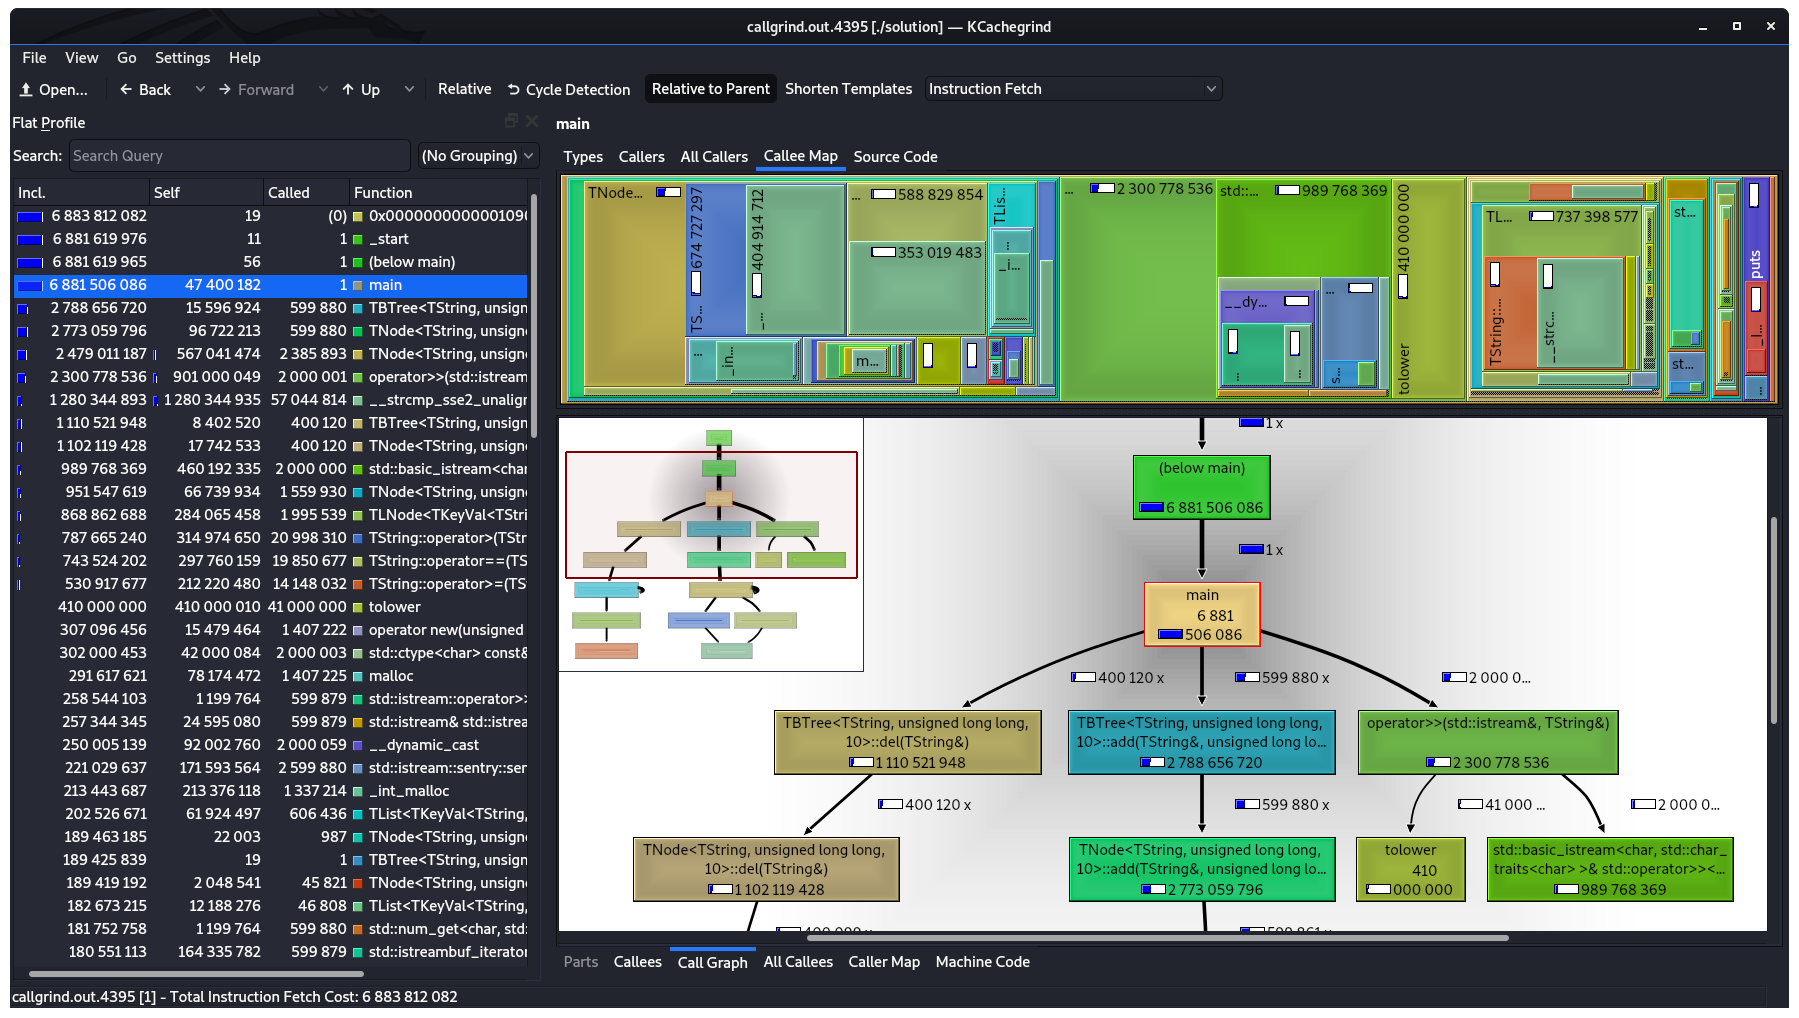
\includegraphics[width=\linewidth]{callgrind}



\subsection*{Дневник этапов написания программы}

1.Написал основную структуру дерева и лист. Проверял вручную правильность работы листа.
2.Написал вставку в дерево вообще нигде не используя delete. Впервые воспользовался отладчиком lldb.
3.После вставки решил заняться удалением. Прежде чем писать удаление написал ко всему диструкторы и проверил в первый раз и отладил все с помощью valgrinda.
4.Реализовал удаление, исправил ошибки с очищением памяти, написал свою менюшку и стринг для того чтобы проверить на чекере. Ошибка выполнения.
5.С помощью lldb и много часов выяснил проблему. Удаление и вставка завершены.
6.Написал сохранение и загрузку дерева. Проверил valgrind'ом и исправил неинициализированные переменные.
7.Все было готово но тайм лимит на 13 тесте. После нескольких дней поисков решения воспользовался профилировщиком 
callgrind и сразу нашел и исправил свой недачет. Программа ускорила свою работу в 3 раза.


\subsection*{Выводы}

Из данной лабораторной работы я вынес, что не обязательно всегда использовать в точности алгоритм, 
как он был рассказан или придуман изначально, а лучше, где это необходимо, немного модифицировать 
алгоритм под ту задачу, которую ты решаешь. К примеру я использовал сортировку подсчетом сразу на
массиве чаров, что, по моему мнению, улучшило читаемость кода и сократило необязательные проблемы.

\end{document}

